\documentclass[11pt]{article}
%Gummi|065|=)
\title{\textbf{Meccano heptagons}}
\author{https://github.com/heptagons/meccano/hepta}
\date{}

\usepackage{amsmath}
\usepackage[pdftex]{graphicx}
\usepackage{listings}
\usepackage{xcolor}
\definecolor{gray}{RGB}{245,245,245}
\usepackage{hyperref}

\lstset{
	backgroundcolor=\color{gray},
	frame=single,
	numbers=left,
	stepnumber=1,
	tabsize=2,
	basicstyle=\ttfamily\small,
	breaklines=true
}

\usepackage[margin=0.75in]{geometry}

\usepackage{graphicx}
\usepackage{hyperref}
\usepackage{multicol}

\begin{document}

\maketitle
\begin{abstract}
We construct meccano\footnote{
\href{https://webspace.science.uu.nl/~hooft101/lectures/meccano.pdf}{Meccano mathematics by `t Hooft }
}
regular heptagons.
We use seven equal strips to build the polygon perimeter and then we attach \textbf{internal diagonals} to make the polygon regular and rigid. Using some
heptagonal identities we deduce three variables $a$, $b$ and $c$ corresponding
to the heptagon side, an internal point of the side and an internal diagonal.
Then we find a closed formula $c = f(a,b)$ and use a program to iterate over $a$ and
$b$ to get $c$ integer which produces prime solutions.
\end{abstract}

\section{Meccano heptagons}

\begin{figure}[htp]
\centering
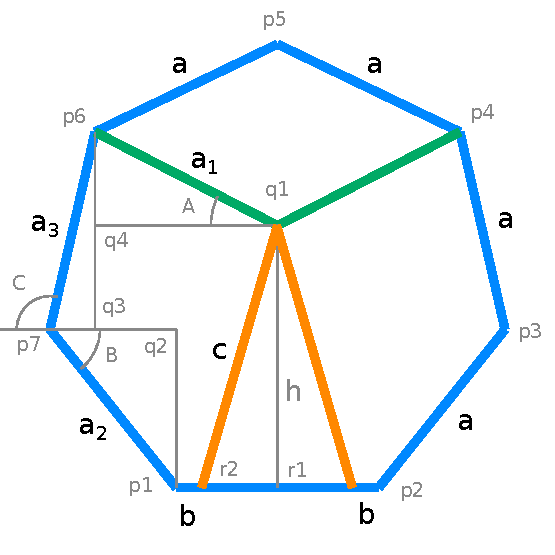
\includegraphics[scale=1]{figs/heptagon_plan.pdf}
\caption{A meccano regular heptagon layout. First we define two integers $a$ and $b$ where $a > 2b$. We look for a third integer $c$ to make the heptagon.}
\label{heptagonplan}
\end{figure}

Consider the regular heptagon in figure \ref{heptagonplan}.
By inspection we identify three angles $A$, $B$ and $C$:

\begin{align*}
A = \frac{\pi}{7},
B = \frac{2\pi}{7},
C = \frac{4\pi}{7}
\end{align*}

Then we find the sines of the angles, noticing that the regular heptagon side is $a = a_1 = a_2 = a_3$:

\begin{align*}
sinA = \frac{\overline{p_6 q_4}}{a_1},
sinB = \frac{\overline{p_1 q_2}}{a_2},
sinC = \frac{\overline{p_6 q_3}}{a_3}
\end{align*}

From the figure the height $h$ corresponds to:

\begin{align*}
h &= \overline{p_1 q_2} + \overline{p_6 q_3} - \overline{p_6 q_4} \\
  &= a_2sinB + a_3sinC - a_1sinA \\
  &= a(-sinA + sinB + sinC)\\
\end{align*}

According to \emph{heptagonal triangles}\footnote{https://en.wikipedia.org/wiki/Heptagonal\_triangle}

\begin{align*}
sinA - sinB - sinC &= -\frac{\sqrt{7}}{2} \\
       \frac{h}{a} &= \frac{\sqrt{7}}{2} \\
                 h &= \frac{\sqrt{7}a}{2}
\end{align*}


Finally we get the $c$ length as a function of lengths $a$ and $b$:

\begin{align*}
c^2 &= h^2 + \overline{r_1 r_2}^2 \\
    &= (\frac{\sqrt{7}a}{2})^2 + (\frac{a - 2b}{2})^2 \\
    &= \frac{7a^2}{4} + \frac{a^2 - 4ab + 4b^2}{4} +  \\
    &= \frac{8a^2 - 4ab + 4b^2}{4}\\
    &= 2a^2 - ab + b^2
\end{align*}

\subsection{Heptagons search}

A valid meccano heptagon needs to have the three lenghts $a$, $b$ and $c$ as integers. With a software routine we look for c to be integer by incrementing the values of $a$ and $b$, where $b < \lceil a/2 \rceil$.

\subsection{Code}

Following code function \texttt{Diagonals} (line 9) find several integer diagonals $c$ in 
function of variables $a$ and $b$. We iterate over $2 \leq a \leq max$ (line 14), then
we iterate over $1 \leq b < \lceil a/2 \rceil$ (line 17). Then we check $c$ is and
integer using the previous formula (lines 18 and 19). We store a solution not 
counting repetitions by scaling (line 20).
\begin{lstlisting}
package hepta

import (
	"math"

	"github.com/heptagons/meccano"
)

func Diagonals(max int) *meccano.Sols {

	sols := &meccano.Sols{}

	bMax, aa := 0, 0
	for a := 2; a <= max; a++ {
		bMax = int(math.Ceil(float64(a) / 2))
		aa = 2*a*a
		for b := 1; b < bMax; b++ {
			f := float64(aa - a*b + b*b)
			if c := int(math.Sqrt(f)); math.Pow(float64(c), 2) == f {
				sols.Add(a, b, c)
			}
		}
	}
	return sols
}\end{lstlisting}

\subsection{Results}
Heptagons prime solutions for $a \leq 450$:
\setlength{\columnsep}{100pt}
\begin{multicols}{2}
\begin{lstlisting}
  1  a=  3 b=  1 c=  4
  2  a=  8 b=  1 c= 11
  3  a= 33 b=  2 c= 46
  4  a= 40 b= 17 c= 53
  5  a= 55 b= 14 c= 74
  6  a= 65 b= 31 c= 86
  7  a= 85 b= 14 c=116
  8  a= 91 b=  2 c=128
  9  a= 95 b=  1 c=134
 10  a= 96 b= 47 c=127
 11  a=105 b= 23 c=142
 12  a=119 b= 46 c=158
 13  a=120 b= 23 c=163
 14  a=133 b= 62 c=176
 15  a=144 b= 41 c=193
 16  a=153 b=  7 c=214
 17  a=161 b= 34 c=218
 18  a=171 b= 34 c=232
 19  a=175 b= 17 c=242
 20  a=176 b= 79 c=233
 21  a=207 b= 94 c=274
 22  a=208 b= 47 c=281
 23  a=225 b= 98 c=298
 24  a=240 b=  7 c=337
 25  a=240 b= 89 c=319
 26  a=253 b= 47 c=344
 27  a=261 b= 62 c=352
 28  a=264 b=  1 c=373
 29  a=275 b= 82 c=368
 30  a=279 b= 41 c=382
 31  a=297 b=119 c=394
 32  a=312 b= 73 c=421
 33  a=319 b=158 c=422
 34  a=320 b= 79 c=431
 35  a=325 b= 23 c=452
 36  a=341 b=142 c=452
 37  a=351 b= 62 c=478
 38  a=360 b= 31 c=499
 39  a=377 b=103 c=506
 40  a=403 b=146 c=536
 41  a=407 b= 73 c=554
 42  a=408 b=167 c=541
 43  a=429 b= 46 c=592
 44  a=429 b=191 c=568
 45  a=435 b= 34 c=604
 46  a=448 b=137 c=599
\end{lstlisting}
\end{multicols}

\subsection{Examples}

\begin{figure}[htp]
\centering
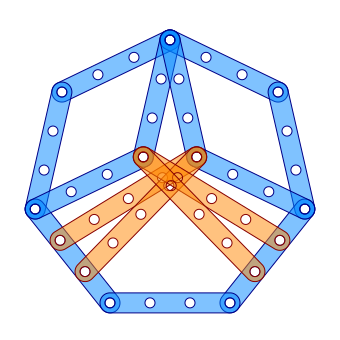
\includegraphics[scale=1]{figs/heptagon-3}
\caption{The first meccano heptagon with values $a=3$, $b=1$ and $c=4$.}
\label{heptagon-3}
\end{figure}

\begin{figure}[htp]
\centering
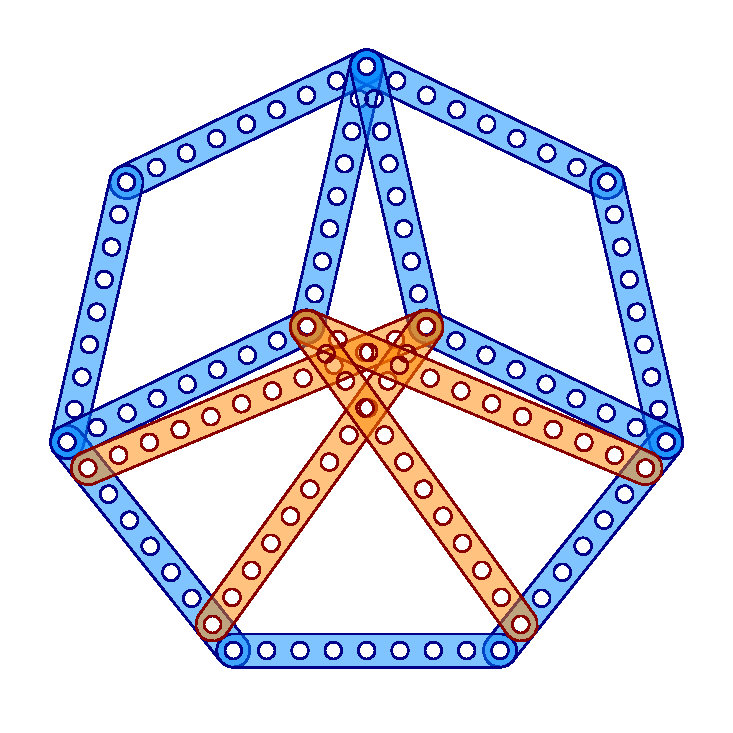
\includegraphics[scale=1]{figs/heptagon-8}
\caption{The second meccano heptagon with values $a=8$, $b=1$ and $c=11$.}
\label{heptagon-8}
\end{figure}

\begin{figure}[htp]
\centering
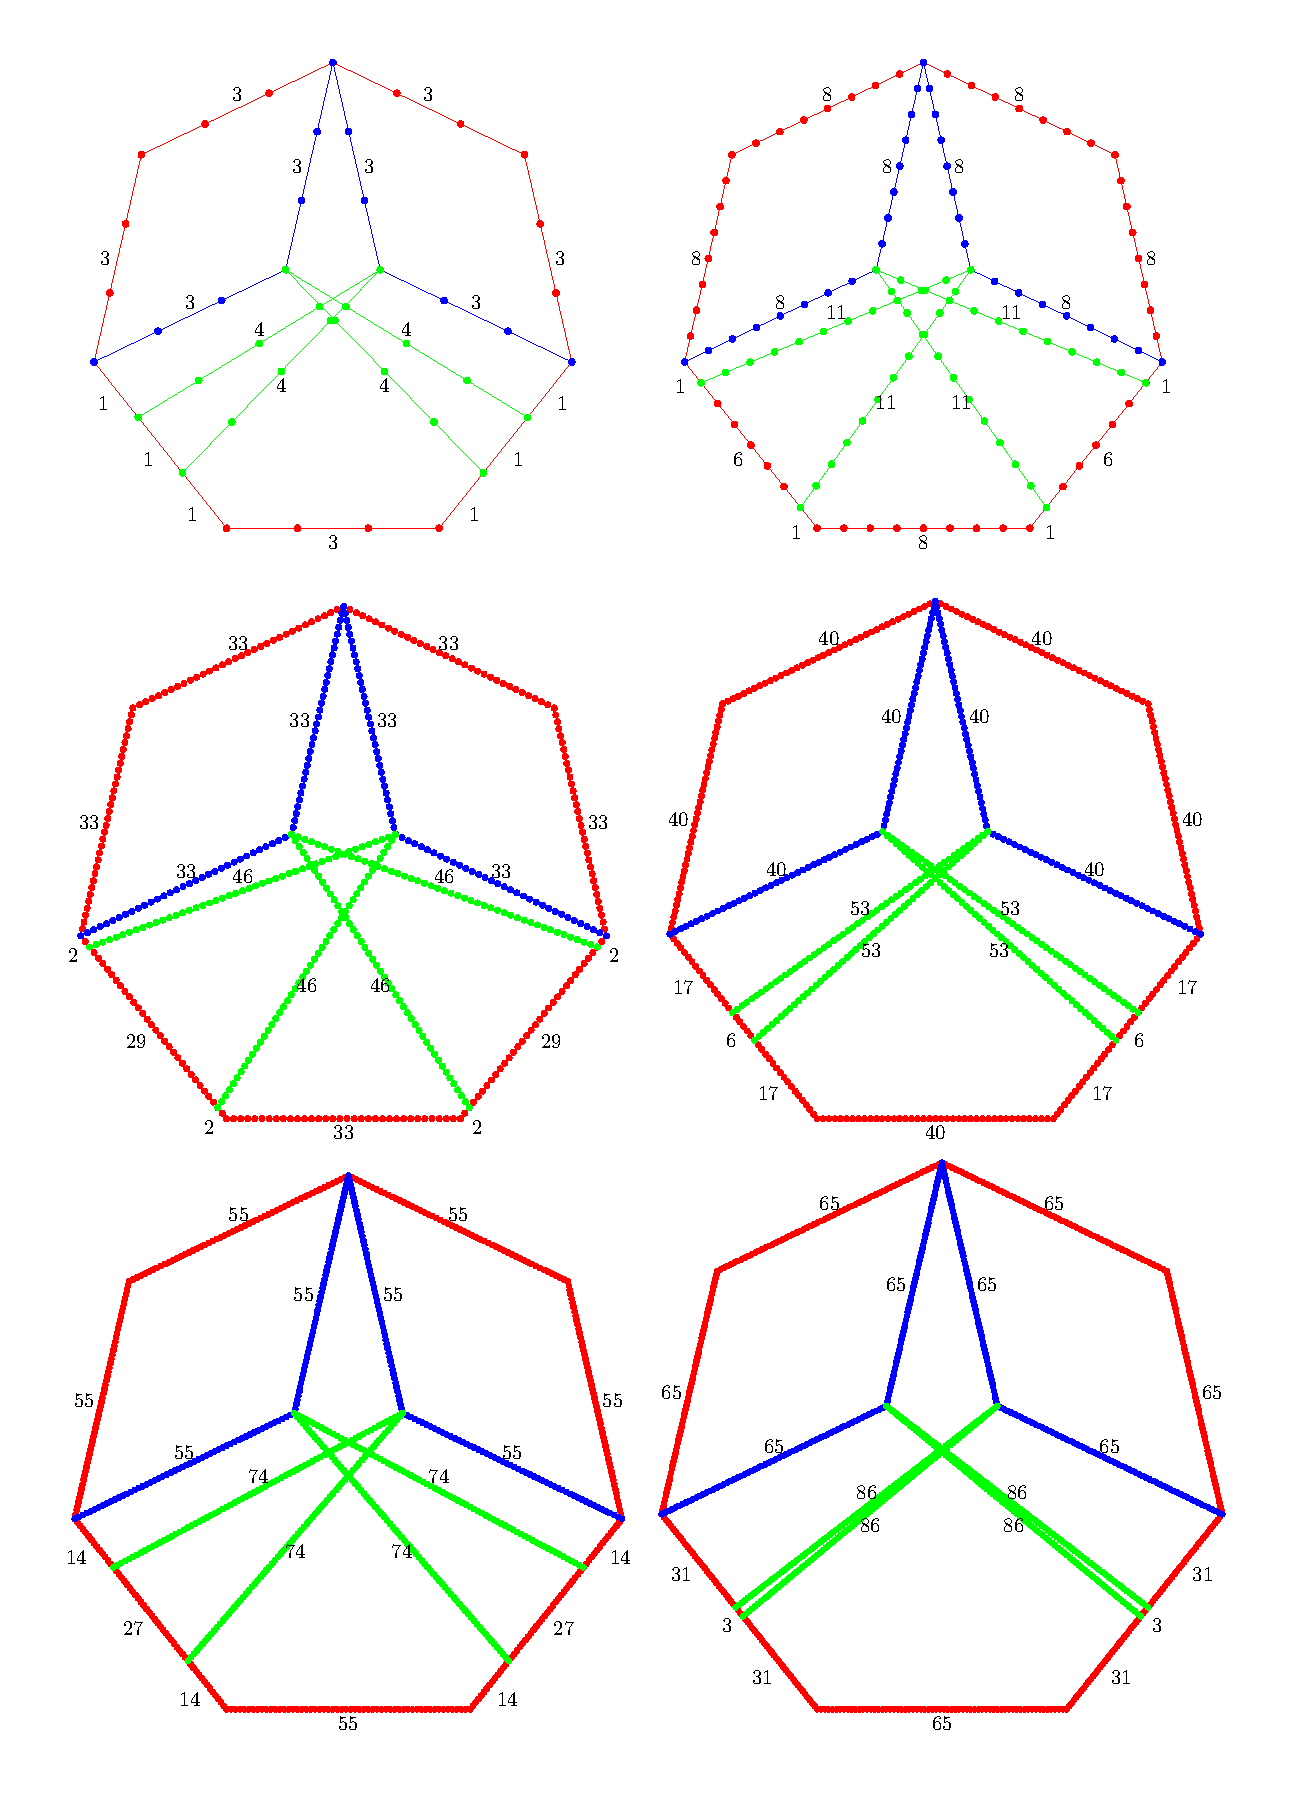
\includegraphics[scale=0.78]{gen}
\caption{The first six prime hexagons $a$ = 3, 8, 33, 40, 55 and 65.}
\label{gen}
\end{figure}

Figures \ref{heptagon-3} and \ref{heptagon-8} show the first two heptagons.
Figure \ref{gen} show the first six heptagons for comparison of growing.

\end{document}

